\subsection{Euclidische co\"ordinaten in het vlak}

In het vlak kies je een paar $(l_1;l_2)$ van snijdende rechten met snijpunt $S$, zie Figuur \ref{fig4.2.2_fig1}.
Herinner, bij een paar is de volgorde van belang.
Op beide rechten kies je een ijk met oorsprong $S$.
Op $l_1$ noteer je $(S;B_1)$ voor die ijk en op $l_2$ noteer je $(S;B_2)$.
Zulke twee geijkte rechten in het vlak noem je een assenstelsel in het vlak.
Het snijpunt $S$ van $l_1$ en $l_2$ noem je de oorsprong van het assenstelsel, vaak aangeduid met $O$.

\begin{center}
\tikzsetfigurename{module4_2_3_assenstelsel}
\begin{tikzpicture}
\draw[-] (-2,-0.4)--(5,1) node[anchor=south,left,yshift=0.2cm]{$l_1$};
\draw[-] (-0.4,-2)--(1,5) node[anchor=south,left]{$l_2$};

\tkzDefPoint(0,0){S}
\tkzDefPoint(2,0.4){B1}
\tkzDefPoint(0.4,2){B2}
\tkzDefPoint(3,0.6){P1}
\tkzDefPoint(0.5,2.5){P2}
\tkzDefPoint(3.5,3.1){P}

\tkzLabelPoint[above,xshift=-0.2cm](S){$S$}
\tkzLabelPoint[below](S){$0$}
\tkzLabelPoint[right](S){$0$}

\tkzLabelPoint[above](B1){$B_1$}
\tkzLabelPoint[below](B1){$1$}
\tkzLabelPoint[left](B2){$B_2$}
\tkzLabelPoint[right](B2){$1$}

\tkzLabelPoint[above,xshift=0.3cm](P1){$P_1$}
\tkzLabelPoint[below](P1){$x$}
\tkzLabelPoint[left](P2){$P_2$}
\tkzLabelPoint[right,yshift=0.2cm](P2){$y$}

\tkzLabelPoint[above](P){$P³(x,y)$}

\tkzDrawSegment[black!60!black](P1,P)
\tkzDrawSegment[black!60!black](P2,P)

\foreach \n in {S,B1,B2,P1,P2,P}
\node at (\n)[circle,fill,inner sep=1.5pt]{};
\end{tikzpicture}
\end{center}

%\gewonefiguur{width=\linewidth}{4_opp_inhoud_an_meetk/inputs/AMTekst2Fig1}

%\begin{figure}[!htb]
%\begin{center}
%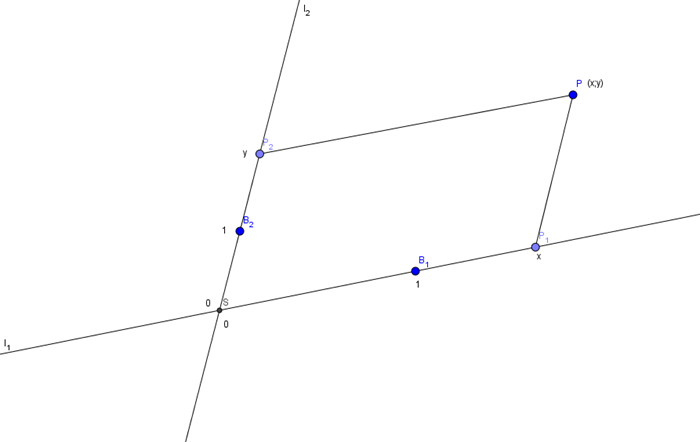
\includegraphics[width=\linewidth]{4_opp_inhoud_an_meetk/inputs/AMTekst2Fig1}
%\caption{}
%\label{fig4.2.2_fig1}
%\end{center}
%\end{figure}

Neem een punt $P$ in het vlak.
Het beeld door $P$ te projecteren evenwijdig aan $l_2$ op $l_1$ noem je $P_1$.
De abscis van $P_1$  op de geijkte rechte $l_1$ is $x$.
Het beeld door $P$ te projecteren evenwijdig aan $l_1$ op $l_2$ noem je $P_2$.
De abscis van $P_2$ op de geijkte rechte $l_2$ is $y$.
Je noemt het paar re\"ele getallen $(x;y)$ de co\"ordinaten van $P$ ten opzichte van het assenstelsel.
Je noteert $\co (P)=(x;y)$.
Ook hier bedoelen we met een paar getallen $(x;y)$ dat de volgorde belang heeft.
In dit geval mogen (en kunnen) de twee getallen $x$ en $y$ gelijk zijn.

Je noemt in deze situatie de geijkte rechte $l_1$ vaak de $x$-as en de geijkte rechte $l_2$ de $y$-as.
Op een tekening noteer je vaak $x$ en $y$ bij die assen en je duidt ook de pijl van de ori\"entatie aan, zoals hieronder.

\begin{center}
\tikzsetfigurename{module4_2_3_assenstelselxy}
\begin{tikzpicture}
\draw[->] (-2,-0.4)--(5,1) node[anchor=south,left,yshift=0.2cm]{$x$};
\draw[->] (-0.4,-2)--(1,5) node[anchor=south,left]{$y$};

\tkzDefPoint(0,0){S}
\tkzDefPoint(2,0.4){B1}
\tkzDefPoint(0.4,2){B2}

\tkzLabelPoint[below](S){$0$}
\tkzLabelPoint[right](S){$0$}

\tkzLabelPoint[below](B1){$1$}
\tkzLabelPoint[right](B2){$1$}

\foreach \n in {S,B1,B2}
\node at (\n)[circle,fill,inner sep=1.5pt]{};
\end{tikzpicture}
\end{center}

%\gewonefiguur{height=5cm}{4_opp_inhoud_an_meetk/inputs/AMTekst2Fig2}

%\begin{figure}[!htb]
%\begin{center}
%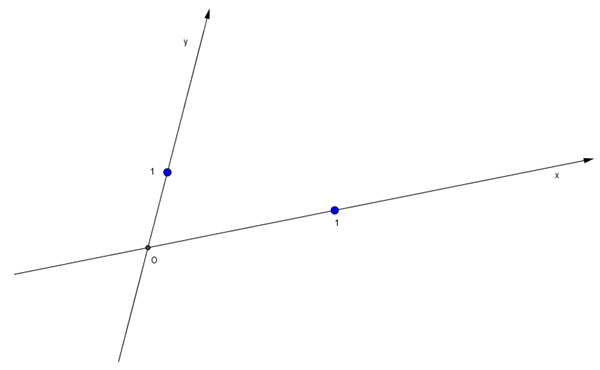
\includegraphics[height=5 cm]{4_opp_inhoud_an_meetk/inputs/AMTekst2Fig2}
%\caption{}
%\label{fig4.2.2_fig2}
%\end{center}
%\end{figure}


\begin{opmerking}
	\begin{itemize}
\item de co\"ordinaten van de oorsprong $O$ zijn $(0;0)$.
\item de co\"ordinaten van punten op de $x$-as zijn van de vorm $(x;0)$.
\item de co\"ordinaten van punten op de $y$-as zijn van de vorm $(0;y)$.
\end{itemize}
\end{opmerking}

Kies een vaste lengte-eenheid (bijvoorbeeld 1 cm).
Een Euclidisch assenstelsel in het vlak is een assenstelsel dat voldoet aan de twee volgende eisen
\begin{itemize}
\item de $x$-as en $y$-as staan loodrecht op elkaar.
\item de geijkte assen $x$ en $y$ komen overeen met de lengte-eenheid.
\end{itemize}
De co\"ordinaten van een punt $P$ in het vlak voorzien van een Euclidisch assenstelsel heten Euclidische co\"ordinaten.
In het vervolg van de cursus (tenzij anders vermeld) gebruiken we enkel Euclidische co\"ordinaten in een vlak.

Vaak teken je een Euclidisch assenstelsel als volgt
\begin{itemize}
\item de $x$-as horizontaal met de positieve richting naar rechts.
\item de $y$-as verticaal met de positieve richting naar boven.
\end{itemize}
In deze ligging is de georiënteerde hoek van de positieve richting van de $x$-as naar de positieve richting van de $y$-as $90^{\circ}$ in tegenwijzerszin, zoals hieronder.
Zulk assenstelsel in het vlak noem je positief geori\"enteerd.


\begin{center}
\tikzsetfigurename{module4_2_3_assenstelselEuclidisch}
\begin{tikzpicture}
\draw[->] (-2,0)--(2,0) node[anchor=south,left,yshift=0.2cm]{$x$};
\draw[->] (0,-2)--(0,2) node[anchor=south,left]{$y$};

\tkzDefPoint(0,0){O}
\tkzDefPoint(0,0){S}
\tkzDefPoint(1,0){A}
\tkzDefPoint(0,1){B}
\tkzDefPoint(-1,0){C}
\tkzDefPoint(3,0){D}
\tkzDefPoint(4,0){E}
\tkzDefPoint(0,-2){F}
\tkzDefPoint(0,-3){G}
\tkzDefPoint(0,4){H}
\tkzDefPoint(0,3){I}
\tkzDefPoint(-1,3){J}
\tkzDefPoint(3,4){K}
\tkzDefPoint(4,-2){L}
\tkzDefPoint(-5,-3){M}
\tkzDefPoint(-5,0){N}

%\tkzDrawSegment[black!60!black,dotted](H,K)
%\tkzDrawSegment[black!60!black,dotted](D,K)
%\tkzDrawSegment[black!60!black,dotted](E,L)
%\tkzDrawSegment[black!60!black,dotted](F,L)	
%\tkzDrawSegment[black!60!black,dotted](G,M)
%\tkzDrawSegment[black!60!black,dotted](N,M)
%\tkzDrawSegment[black!60!black,dotted](C,J)
%\tkzDrawSegment[black!60!black,dotted](I,J)
%
\tkzLabelPoint[below,xshift=-0.2cm](S){$0$}
\tkzLabelPoint[below](A){$1$}
%\tkzLabelPoint[below](D){$3$}
%\tkzLabelPoint[above](E){$4$}
%\tkzLabelPoint[below](C){$-1$}
%\tkzLabelPoint[above](N){$-5$}
\tkzLabelPoint[left](B){$1$}
%\tkzLabelPoint[right](I){$3$}
%\tkzLabelPoint[left](H){$4$}
%\tkzLabelPoint[left](F){$-2$}
%\tkzLabelPoint[right](G){$-3$}
%
%\tkzLabelPoint[left](M){$T$}
%\tkzLabelPoint[above](J){$Q$}
%\tkzLabelPoint[above](K){$P$}
%\tkzLabelPoint[below](L){$R$}

\foreach \n in {A,B,O}
\node at (\n)[circle,fill,inner sep=1.5pt]{};

\pic [draw, ->, "", angle eccentricity=0.5] {angle = A--O--B};

\end{tikzpicture}	
\end{center}


%\gewonefiguur{height=5cm}{4_opp_inhoud_an_meetk/inputs/AMTekst2Fig3}

%\begin{figure}[!htb]
%\begin{center}
%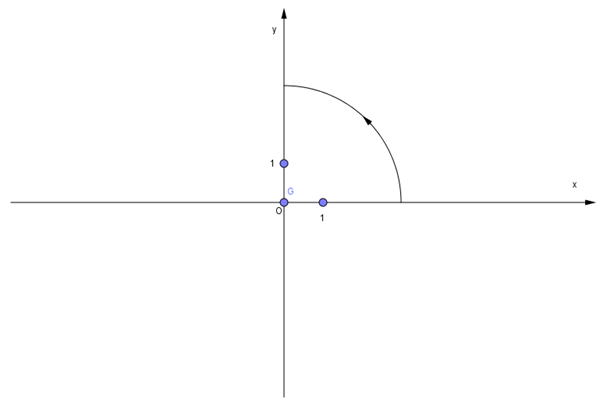
\includegraphics[height=5 cm]{4_opp_inhoud_an_meetk/inputs/AMTekst2Fig3}
%\caption{}
%\label{fig4.2.2_fig3}
%\end{center}
%\end{figure}

Op de volgende figuur zijn in een Euclidisch assenstelsel met die ligging de volgende punten met hun co\"ordinaten aangeduidt: $P(3;4)$, $Q(-1;3)$, $R(4;-2)$ en $T(-5;-3)$.

\begin{center}
	\tikzsetfigurename{module4_2_3_assenstelselEuclidisch_cdn}
\begin{tikzpicture}
\draw[->] (-5,0)--(5,0) node[anchor=south,left,yshift=0.2cm]{$x$};
\draw[->] (0,-5)--(0,5) node[anchor=south,left]{$y$};

\tkzDefPoint(0,0){O}
\tkzDefPoint(0,0){S}
\tkzDefPoint(1,0){A}
\tkzDefPoint(0,1){B}
\tkzDefPoint(-1,0){C}
\tkzDefPoint(3,0){D}
\tkzDefPoint(4,0){E}
\tkzDefPoint(0,-2){F}
\tkzDefPoint(0,-3){G}
\tkzDefPoint(0,4){H}
\tkzDefPoint(0,3){I}
\tkzDefPoint(-1,3){J}
\tkzDefPoint(3,4){K}
\tkzDefPoint(4,-2){L}
\tkzDefPoint(-5,-3){M}
\tkzDefPoint(-5,0){N}

\tkzDrawSegment[black!60!black,dotted](H,K)
\tkzDrawSegment[black!60!black,dotted](D,K)
\tkzDrawSegment[black!60!black,dotted](E,L)
\tkzDrawSegment[black!60!black,dotted](F,L)	
\tkzDrawSegment[black!60!black,dotted](G,M)
\tkzDrawSegment[black!60!black,dotted](N,M)
\tkzDrawSegment[black!60!black,dotted](C,J)
\tkzDrawSegment[black!60!black,dotted](I,J)

\tkzLabelPoint[below,xshift=-0.2cm](S){$0$}
\tkzLabelPoint[below](A){$1$}
\tkzLabelPoint[below](D){$3$}
\tkzLabelPoint[above](E){$4$}
\tkzLabelPoint[below](C){$-1$}
\tkzLabelPoint[above](N){$-5$}
\tkzLabelPoint[left](B){$1$}
\tkzLabelPoint[right](I){$3$}
\tkzLabelPoint[left](H){$4$}
\tkzLabelPoint[left](F){$-2$}
\tkzLabelPoint[right](G){$-3$}

\tkzLabelPoint[left](M){$T$}
\tkzLabelPoint[above](J){$Q$}
\tkzLabelPoint[above](K){$P$}
\tkzLabelPoint[below](L){$R$}

\foreach \n in {A,B,C,D,E,F,G,H,I,J,K,L,M,N,O}
\node at (\n)[circle,fill,inner sep=1.5pt]{};

\end{tikzpicture}	
\end{center}

%\gewonefiguur{width=.7\linewidth}{4_opp_inhoud_an_meetk/inputs/AMTekst2Fig4}

%\begin{figure}[!htb]
%\begin{center}
%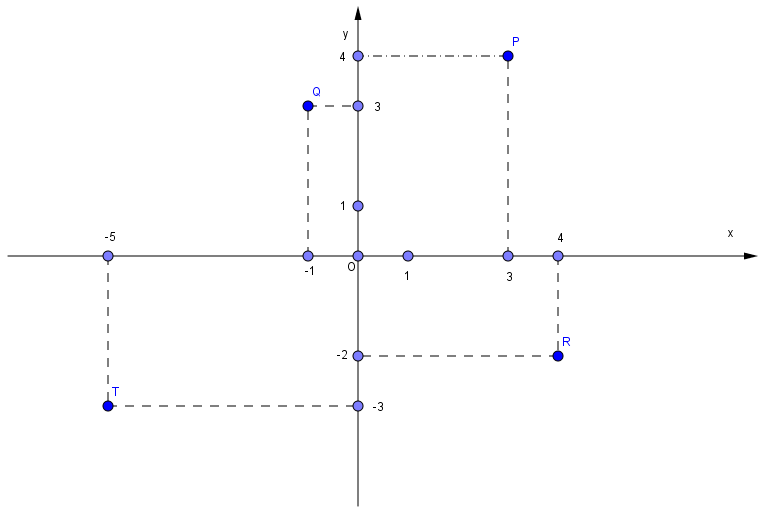
\includegraphics[width=.7\linewidth]{4_opp_inhoud_an_meetk/inputs/AMTekst2Fig4}
%\caption{}
%\label{fig4.2.2_fig4}
%\end{center}
%\end{figure}

Een assenstelsel verdeelt het vlak in 4 delen.
Je noemt dat de kwadranten.
Deze nummer je in tegenwijzerszin. 
Je start met het deel waar $x$ en $y$ allebei positief zijn.
Dat noem je het eerste kwadrant, zoals in de figuur hieronder.

\begin{minipage}{.5\linewidth}
%\gewonefiguur{width=.5\linewidth}{4_opp_inhoud_an_meetk/inputs/AMTekst2Fig5}
\begin{center}
\begin{tabular}{c|c|c}
	Kwadrant & $x$ & $y$ \\
	\hline
	I & + & + \\
	II & - & + \\
	III & - & - \\
	IV & + & - \\
\end{tabular}	
\end{center}
\end{minipage}
\begin{minipage}{.5\linewidth}
\begin{center}
	\tikzsetfigurename{module4_2_3_kwadranten}
\begin{tikzpicture}
\coordinate (a) at (0,0);
\coordinate (b) at (2,0);
\coordinate (c) at (0,2);

\draw[->] (-3,0)--(3,0) node[anchor=south,left,yshift=0.2cm]{$x$};
\draw[->] (0,-3)--(0,3) node[anchor=south,left]{$y$};

\tkzDefPoint(0,0){S}
\tkzDefPoint(1,0){B1}
\tkzDefPoint(0,1){B2}

\tkzLabelPoint[below,xshift=-0.1cm](S){$0$}
\tkzLabelPoint[right,yshift=0.1cm](S){$0$}

\tkzLabelPoint[below](B1){$1$}
\tkzLabelPoint[right](B2){$1$}

\foreach \n in {S,B1,B2}
\node at (\n)[circle,fill,inner sep=1.5pt]{};

%	\node[draw,align=right] at (1,2) {Kwadrant I};
%	\node[draw,align=left] at (-1,2) {Kwadrant II};
%	\node[draw,align=left] at (-1,-1) {Kwadrant III};
%	\node[draw,align=right] at (1,-1) {Kwadrant IV};

\node[] at (1.5,1.5) {Kwadrant I};
\node[] at (-1.5,1.5) {Kwadrant II};
\node[] at (-1.5,-1.5) {Kwadrant III};
\node[] at (1.5,-1.5) {Kwadrant IV};

\end{tikzpicture}	
\end{center}
\end{minipage}
